\documentclass[a4paper]{article}

\addtolength{\hoffset}{-2.25cm}
\addtolength{\textwidth}{4.5cm}
\addtolength{\voffset}{-3.25cm}
\addtolength{\textheight}{5cm}
\setlength{\parskip}{0pt}
\setlength{\parindent}{0in}

%----------------------------------------------------------------------------------------
%	PACKAGES AND OTHER DOCUMENT CONFIGURATIONS
%----------------------------------------------------------------------------------------

\usepackage{blindtext} % Package to generate dummy text
\usepackage{charter} % Use the Charter font
\usepackage[utf8]{inputenc} % Use UTF-8 encoding
\usepackage{microtype} % Slightly tweak font spacing for aesthetics
\usepackage[english]{babel} % Language hyphenation and typographical rules
\usepackage{amsthm, amsmath, amssymb} % Mathematical typesetting
\usepackage{float} % Improved interface for floating objects
\usepackage[final, colorlinks = true,
            linkcolor = black,
            citecolor = black]{hyperref} % For hyperlinks in the PDF
\usepackage{graphicx, multicol} % Enhanced support for graphics
\usepackage{xcolor} % Driver-independent color extensions
\usepackage{marvosym, wasysym} % More symbols
\usepackage{rotating} % Rotation tools
\usepackage{censor} % Facilities for controlling restricted text
\usepackage{listings} % Environment for non-formatted code, !uses style file!
\usepackage{pseudocode} % Environment for specifying algorithms in a natural way
 % Environment for f-structures, !uses style file!
\usepackage{booktabs} % Enhances quality of tables
\usepackage{tikz-qtree} % Easy tree drawing tool
 % Configuration for b-trees and b+-trees, !uses style file!
\usepackage[backend=biber,style=numeric,
            sorting=nyt]{biblatex} % Complete reimplementation of bibliographic facilities
\addbibresource{ecl.bib}
\usepackage{csquotes} % Context sensitive quotation facilities
\usepackage[yyyymmdd]{datetime} % Uses YEAR-MONTH-DAY format for dates
\renewcommand{\dateseparator}{-} % Sets date separator to '-'
\usepackage{fancyhdr} % Headers and footers
\pagestyle{fancy} % All pages have headers and footers
\fancyhead{}\renewcommand{\headrulewidth}{0pt} % Blank out the default header
\fancyfoot[L]{} % Custom footer text
\fancyfoot[C]{} % Custom footer text
\fancyfoot[R]{\thepage} % Custom footer text
\newcommand{\note}[1]{\marginpar{\scriptsize \textcolor{red}{#1}}} % Enables comments in red on margin
\usepackage{mathtools}
\usepackage{amsmath}
\DeclarePairedDelimiter\abs{\lvert}{\rvert}%
\usepackage{cancel}
\usepackage{minted}
\usepackage{float}
\usepackage{caption}
\usepackage{subcaption}
%-------------------------------

%----------------------------------------------------------------------------------------

%-------------------------------
%	ENVIRONMENT SECTION
%-------------------------------
\pagestyle{fancy}
\usepackage{mdframed}

\usepackage[sfdefault]{FiraSans} %% option 'sfdefault' activates Fira Sans as the default text font
\usepackage[T1]{fontenc}
\renewcommand*\oldstylenums[1]{{\firaoldstyle #1}}


% remove numbering from sections
\usepackage{titlesec}
\titleformat{\section}{\normalfont\Large\bfseries}{}{0pt}{}



%-------------------------------------------------------------------------------------------
%	CUSTOM COMMANDS
%-------------------------------
\newcommand{\gaussian}{\frac{1}{\sigma\sqrt{2\pi}}\exp\left(- \frac{(x-\mu)^2}{2\sigma^2}\right)}
\newcommand{\R}{\mathbb R}

\def\inline{\lstinline[basicstyle=\ttfamily,keywordstyle={}]}


\begin{document}


%-------------------------------
%	TITLE SECTION
%-------------------------------

\fancyhead[C]{}
\hrule \medskip % Upper rule
\begin{minipage}{0.295\textwidth}
  \raggedright
  \footnotesize
  Francisco Javier Sáez Maldonado \hfill\\
  franciscojavier.saez@estudiante.uam.es
  \hfill\\
\end{minipage}
\begin{minipage}{0.4\textwidth}
  \centering
  \large
  Image Classification. CNN architectures. Transfer Learning\\
  \normalsize
  Deep Learning for Image and Video Processing\\
\end{minipage}
\begin{minipage}{0.295\textwidth}
  \raggedleft
  \today\hfill\\
\end{minipage}
\medskip\hrule

%-------------------------------
%	CONTENTS
%-------------------------------

\section{Simple CNN}

In this first section, we will present the results obtained by a Simple CNN classifying the digits in the MNIST dataset. Let show some properties about the images in this dataset:

\begin{itemize}
  \item Train and validation set sizes in MNIST:
        \begin{table}[H]
          \centering
          \begin{tabular}{l|rrrr}
                       & \multicolumn{1}{l}{Image height} & \multicolumn{1}{l}{Image width} & \multicolumn{1}{l}{Number of Channels} & \multicolumn{1}{l}{Number of samples} \\ \hline
            Train      & 28                               & 28                              & 1                                      & 60000                                 \\
            Validation & 28                               & 28                              & 1                                      & 10000
          \end{tabular}
        \end{table}
  \item Number of trainable parameters of the simple CNN model:
        \begin{table}[H]
          \centering
          \begin{tabular}{l|r}
                       & \multicolumn{1}{l}{Number of trainable parameters} \\  \hline
            Simple CNN & 813802
          \end{tabular}
        \end{table}
  \item Show the learning curves for the first \(10\) epochs. Also indicate the best accuracy obtained and the epoch in which this accuracy is obtained. Comment the conclusions about the evolution of the \emph{loss} in both training and validation sets, with respect to the possible \emph{high-bias} or \emph{overfitting} problems. Would training the model for more epoch improve the performance of the model?
        \begin{table}[H]
          \centering
          \begin{tabular}{l|rr}
                       & \multicolumn{1}{l}{Highest accuracy (validation)} & Epoch with highest accuracy \\ \hline
            Simple CNN & 99.01                                             & 10
          \end{tabular}
        \end{table}
        As we can see, our model gets a result that is close to $100\%$ accuracy, which means that our model is capable of classifying almost all validation images correctly. Let us see the learning curves:
        \begin{figure}[H]
          \centering
          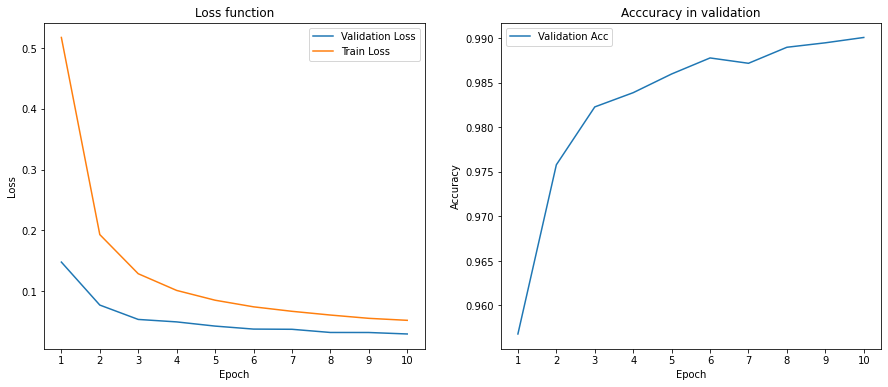
\includegraphics[scale = 0.5]{Figures/LearningCurvesSimpleCNN.png}
          \caption{Learning curves for the Simple CNN model.}
        \end{figure}

        As we can see, the loss function values are always lower in the validation set. This \textbf{makes sense} due to the \textbf{dropout}. While training, some neurons are deactivated because of the dropout, leading to \emph{worse} outputs in each batch and, thus, higher loss values. When the validation is performed, \textbf{all the weights} are used (dropout is off), so a better middle representation is obtained resulting in a lower loss. In general, we can say that dropout helps us to \textbf{avoid overfitting}. \\

        The value of the loss function in both train and validation sets  \textbf{always decreases}, so we can not say that our model is overfitting yet. Since we are not overfitting yet and the learning curves have not \emph{flattened} (become almost constant), we state that it would be \textbf{beneficial} to the model to resume the training for a few more epochs. In fact, we tested this and obtained the following results:

        \begin{figure}[H]
          \centering
          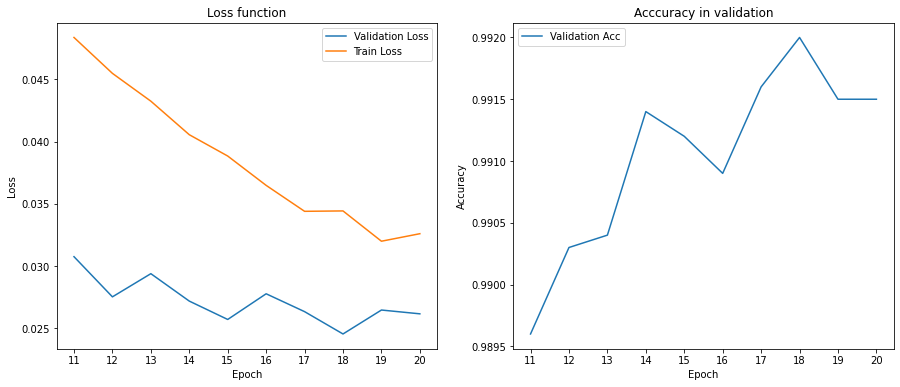
\includegraphics[scale = 0.5]{Figures/LearningCurvesSimpleCNN-Longer.png}
          \caption{Learning curves for the following \(10\) epochs.}
        \end{figure}

        As we can observe (also looking at the \(y\) axis values), the decrease in the loss function and the increase in the accuracy are not relevant. The loss function values in the \emph{train set} even increases sometimes in the last epochs, indicating that the model is possibly already \textbf{overfitting}.\\

        We have not observed any \textbf{high-bias} problems in any of the cases.

  \item Show the obtained confusion matrix. Given this confusion matrix, which are the most two confused classes?


        \begin{figure}[H]
          \centering
          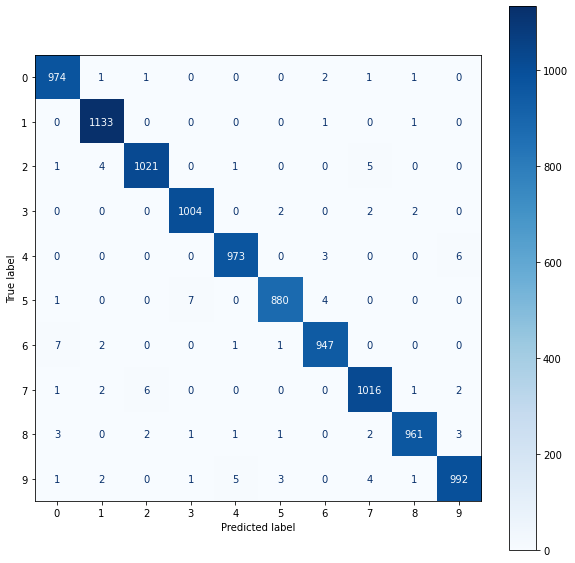
\includegraphics[scale = 0.5]{Figures/SimpleCNNConfusion.png}
          \caption{Confusion matrix of the Simple CNN model in MNIST dataset.}
        \end{figure}

        As we can see in the confusion matrix, there are two pairs of numbers that are the most confused:

        \begin{itemize}
          \item \(6-0\). In this case, this confusion is justified due to the rounded shape of both numbers, and if the upper side of the number \(6\) is not \emph{separated} enough from the rest of the number, the model could be confused.
          \item \(5-3\). These two numbers are identical in their lower half and they both have an \emph{"horizontal"} line on the upper half, so the confusion might be justified.
        \end{itemize}

  \item Comment the differences between the \emph{t-SNE} chart of the representation of the final and intermediate layers of the CNN applied to the validation set. Consider the distance and dispersion between clusters in both representations and its relation with the capability of obtaining a correct classification of the samples.\\

        Let us  firstly present the \emph{t-SNE} representations that we have obtained:

        \begin{figure}[H]
          \centering
          \begin{subfigure}{.5\textwidth}
            \centering
            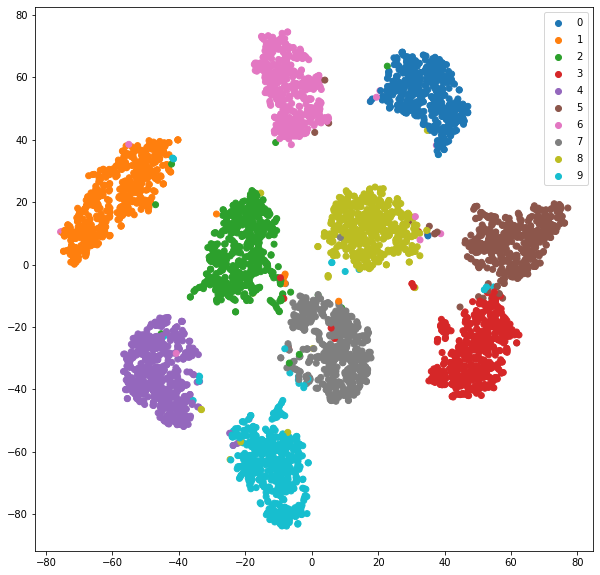
\includegraphics[width=\linewidth]{Figures/SimpleCNN-representation-intermediate.png}
            \caption{\emph{Intermediate Representation}}
            \label{fig:tsne:1}
          \end{subfigure}%
          \begin{subfigure}{.5\textwidth}
            \centering
            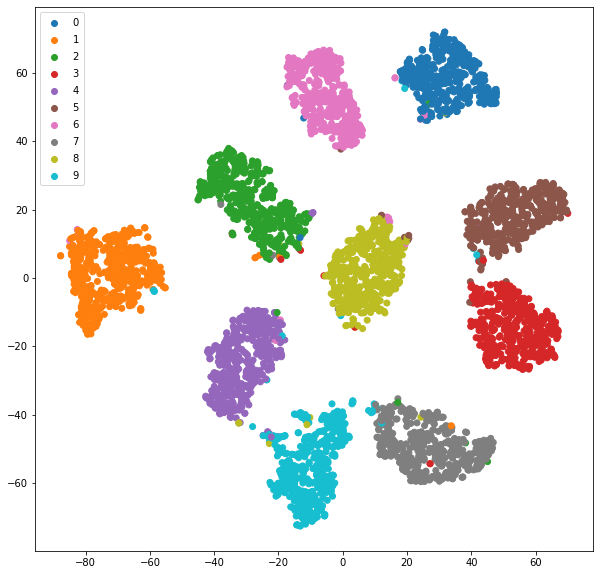
\includegraphics[width=\linewidth]{Figures/SimpleCNN-representation-outputs.png}
            \caption{Output representation}
            \label{fig:tsne:2}
          \end{subfigure}
          \caption{\emph{t-SNE} representations.}
          \label{fig:tsne}
        \end{figure}

        Clearly, the \textbf{output} \emph{t-SNE} has more inter-cluster distance and less dispersion in each cluster, so using this representation would provide better results. \textbf{However}, we could perfectly use the intermediate representations since we see that the clusters are already \textbf{well differentiated} in the intermediate representations. It would be useful to use this intermediate representation if we needed a faster system which also has a good performance.

  \item Given the differences between the \emph{t-SNE} representation in the different layers, and given the architecture of the CNN, identify the layer of the CNN in which the features are extracted and propose a solution to reduce the Network's complexity with a low penalty in classification accuracy.

        Having a look at the architecture of \emph{SimpleCNN}, we observe that the intermediate features are obtained \textbf{after the first linear layer}. Furthermore, the features are obtained in the \textbf{convolutional layers} and refined with the first linear layer. As we just saw in Figure \ref{fig:tsne}, the difference between the representations is not huge in terms of clustering separability (a nonlinear model could separate the data quite well since there is a fair amount of distance between the clusters), so \textbf{erasing the last linear layer} would be a way to reduce the network's complexity with a low penalty in classification.

        Further study on the intermediate representations obtained by each \emph{convolutional layer} should be done in order to determine if some convolutional layers could be removed.
\end{itemize}

\newpage

\section{AlexNet}

In this section, we propose a \textbf{reduced} implementation of the famous \emph{AlexNet}, and we test it in the dataset \textbf{CIFAR10}.

\begin{itemize}
  \item Include the code used to define the \inline{AlexNet} class.
        The code used to implement is the following:
        \begin{minted}{Python}
          class AlexNet(nn.Module):
    def __init__(self, output_dim):
        super().__init__()
        
        self.features = nn.Sequential(
            # First convolutional layer. Use 5x5 kernel instead of 11x11
            # Recall that image input will be 32x32!

            # 5x5 layers
            #-----------
            #in_channels, out_channels, kernel_size, stride, padding
            nn.Conv2d(3, 48, 5, 2, 2), 
            nn.MaxPool2d(2), #kernel_size
            nn.ReLU(inplace = True),
            # Subsampling is only performed by 2x2 max pooling layers 
            # (not with stride in the  convolutional layers)
            nn.Conv2d(48,128,5,1,2),
            nn.MaxPool2d(2), #kernel_size
            nn.ReLU(inplace = True),

            # 3x3 layers
            #-----------
            # First 3x3 layer
            nn.Conv2d(128,192,3,1,1),
            nn.ReLU(inplace = True),
            # Second 3x3 layer
            nn.Conv2d(192,192,3,1,1),
            nn.ReLU(inplace = True),
            # Third 3x3 layer
            nn.Conv2d(192,128,3,1,1),
            nn.MaxPool2d(2),
            nn.ReLU(inplace = True)
        )
        
        self.classifier = nn.Sequential(
            # First linear layer
            nn.Dropout(0.5),
            nn.Linear(128 * 2 * 2, 2048), # final conv layer resolution 2x2
            nn.ReLU(inplace = True),
            # Second dropout
            nn.Dropout(0,5),
            # second linear layer
            nn.Linear(2048, 2048),
            nn.ReLU(inplace = True),
            # Last Linear layer. No ReLU
            nn.Linear(2048, output_dim)
        )

    def forward(self, x):
        x = self.features(x)
        interm_features = x.view(x.shape[0], -1)
        x = self.classifier(interm_features)
        return x, interm_features
        \end{minted}

        In this case, we are using \textbf{two sequential blocks} in order to simplify the code of the \inline{forward} method.
  \item Number of parameters in AlexNet
        \begin{table}[H]
          \centering
          \begin{tabular}{l|r}
                    & \multicolumn{1}{l}{Number of trainable parameters} \\ \hline
            AlexNet & 6.199.498
          \end{tabular}
        \end{table}
  \item Learning curves for the first \(15\) epochs. Also indicate the best accuracy obtained and the epoch in which this accuracy is obtained. Comment the conclusions about the evolution of the \emph{loss} function in both train and test sets. Comment the behavior of this function after epoch \(10\). Would training the model for more epoch improve the performance of the model? \\

        Firstly, we see that the highest accuracy in the validation set is the following:
        \begin{table}[H]
          \centering
          \begin{tabular}{l|rr}
                    & \multicolumn{1}{l}{Highest accuracy (validation)} & Epoch with highest accuracy \\ \hline
            AlexNet & 0.72                                              & 14
          \end{tabular}
        \end{table}
        We now plot and analyze the learning curves:
        \begin{figure}[H]
          \centering
          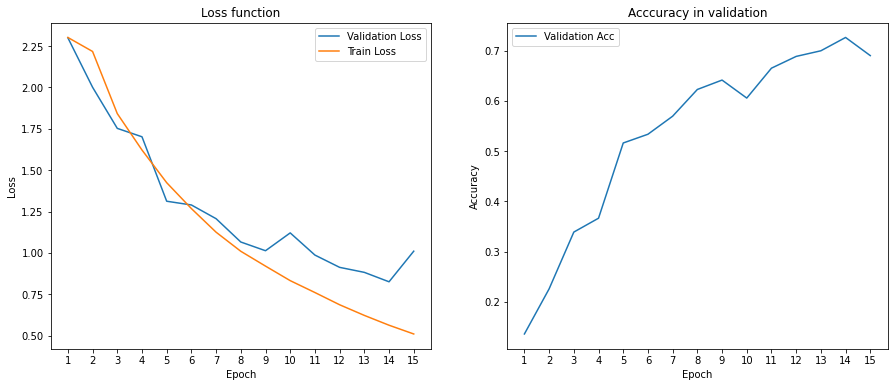
\includegraphics[scale = 0.5]{Figures/AlexNet-LearningCurves.png}
          \caption{Reduced AlexNet: learning curves for the first \(15\) epochs.}
        \end{figure}

        As we can see, after epoch \(10\) we see that the pace of decrease in the loss function in the validation set is much slower than in the previous epochs, which means that our model is already overfitting. Also, as we can see, the increase in the validation accuracy from epoch \(10\) is much lower than the increase in the previous epochs. With this information, we can state that training the model for more epochs \textbf{would not} help our model to obtain better accuracy results, since the model would overfit  the train set.

  \item Show and comment the confusion matrix, taking into account the features of each class images.\\
        \begin{figure}[H]
          \centering
          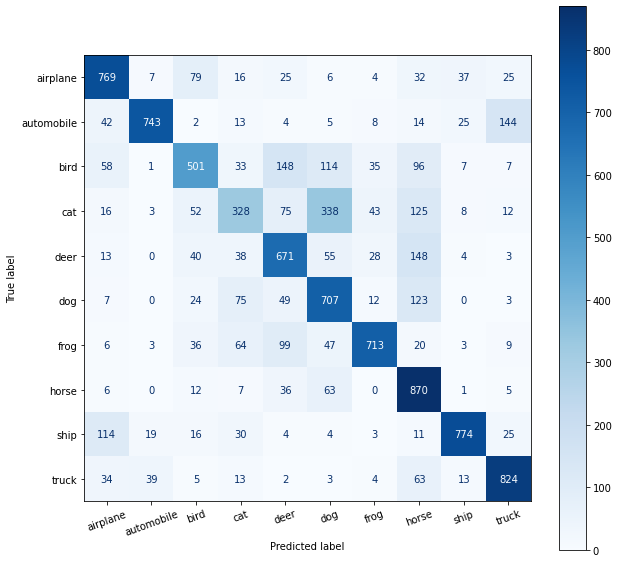
\includegraphics[scale = 0.4]{Figures/AlexNet-Confusion.png}
          \caption{Confusion matrix of Reduced AlexNet in CIFAR10 dataset.}
        \end{figure}

        As we can observe, this confusion matrix shows quite worse results than the one presented for the \emph{MNIST} model, which makes sense if we have a look at the accuracies of each of the models.

        We can comment the classes that are most confused:

        \begin{itemize}
          \item \emph{Automobile-truck}: The similarity between these two classes is high, since they are both vehicles and have similar features such as rounded shapes (wheels) and defined edges (structure of the vehicle).
          \item \emph{Cat-Dog}: both animals have approximately same size and similar facial features, although a human could easily distinguish them.
          \item \emph{Bird-Deer}: this confusion does not make much sense, since the sizes and anatomy of both animals are quite different. The only relation that we could find between the classes is that probably the images of both classes have a \emph{similar background} (surrounded by nature).
          \item \emph{Horse-Deer}: In this case, the resemblance between the two represented animals is much higher, so the confusion makes sense.
        \end{itemize}
  \item Show the \emph{t-SNE} representations for the output layer of the network and analyze them taking into account the aspect of the different class images. Compare the results with the representations obtained in the \textbf{MNIST}.\\ dataset.\\

        The representations obtained by the output class are the following:
        \begin{figure}[H]
          \centering
          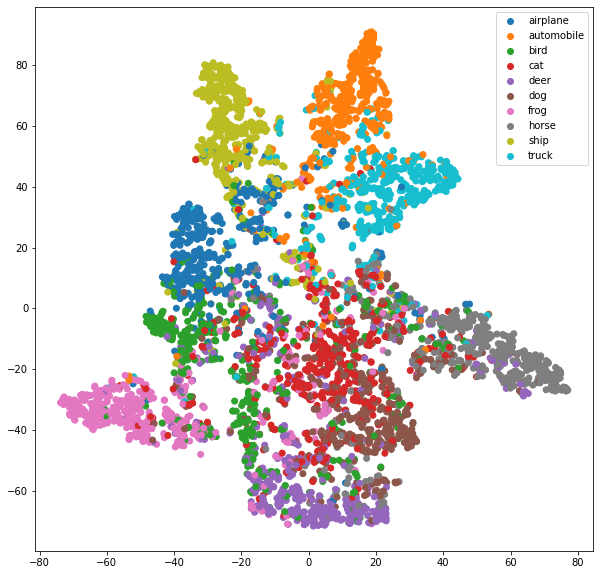
\includegraphics[scale = 0.5]{Figures/AlexNet-tSNE.png}
          \caption{Reduced AlexNet representations by \emph{t-SNE}.}
        \end{figure}

        As it can be appreciated after a quick look, the clusters of representations are \textbf{much worse} separated than in the previous case. It seems different classes are grouped in \emph{separated} groups, however the amount of noise appearing in each of those groups is much higher than it happened in the \emph{MNIST} case. Furthermore, some of the classes that were being confused have really close \emph{t-SNE} representations (in terms of \(\mathbb R^2\) distance), as it happens in the case of the classes \emph{Cat-Dog} or \emph{Automobile-Truck}.\\

        In order to improve the robustness of the model in the representation-learning stage, we should probably use data augmentation techniques in order to give the model more examples of the desired classes.
\end{itemize}

\section{Transfer learning}

In this last section, we study the effect of using the pre-trained feature extraction layers of a model in a different problem to see if it provides a good starting point for the new problem. We will use the Alien vs Predator dataset from Kaggle.


\begin{itemize}
  \item Show the precisions obtained for the different analyzed alternatives.
        \begin{table}[H]
          \begin{tabular}{l|llll}
                     & Trained from zero        & Pretrained + SVM          & \begin{tabular}[c]{@{}l@{}}Finetuning (no data\\ augmentation)\end{tabular} & Finetuning (data augmentation) \\ \hline
            Accuracy & \multicolumn{1}{r}{0.72} & \multicolumn{1}{r}{0.905} & \multicolumn{1}{r}{0.935}                                                   & \multicolumn{1}{r}{0.95}
          \end{tabular}
          \caption{Obtained results in transfer learning in the Alien dataset.}
          \label{table:transfer}
        \end{table}

        The Table \ref{table:transfer} represents the results obtained in each of the stages of the transfer learning process performed. The results show what we expected:
        \begin{enumerate}
          \item Firstly, the trained from scratch model performs worse than using a pretrained model (with no training at all) to extract features and use a classifier on top of that model.
          \item Then, it is shown how the performance improves when we \emph{freeze} all layers but the last one and train that layer for a few epochs (which is known as finetuning).
          \item Lastly, we check the positive effect of applying data augmentation when training both the last linear layer and the classifier, obtaining the highest accuracy.
        \end{enumerate}
        All this results were expected, since it is known that ResNet (network used as feature extractor) is one of the most powerful CNN architectures and finetuning the last layers adapts the pretrained weights to improve the performance on a new problem.
  \item Compare the \emph{t-SNE} representations of the different alternatives. From these representations, comment the difference in terms of linear separability and the accuracy of this linear separability.\\

        We plot the \emph{t-SNE} representations, using a \textbf{linear model} to try to separate the classes.
        \begin{figure}[H]
          \centering
          %\centering % Not needed
          \begin{subfigure}[b]{0.49\columnwidth}
            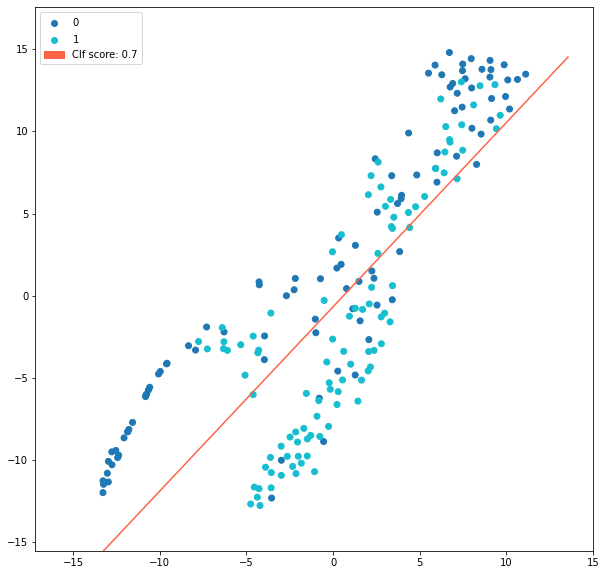
\includegraphics[width=\textwidth]{Figures/transfer-scratch.png}
            \caption{Trained from scratch}
            \label{fig:scratch}
          \end{subfigure}
          \hfill
          \begin{subfigure}[b]{0.49\columnwidth}
            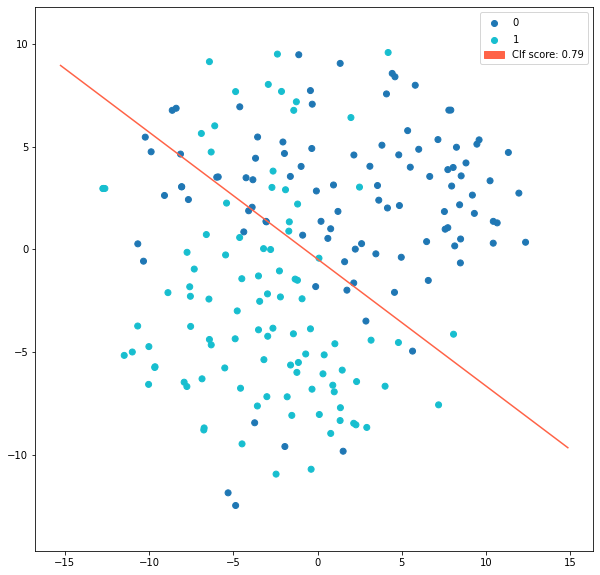
\includegraphics[width=\textwidth]{Figures/transfer-svm.png}
            \caption{ResNet + SVM}
            \label{fig:svm}
          \end{subfigure}
          %% leave a blank line to create a line break

          \begin{subfigure}[b]{0.49\columnwidth}
            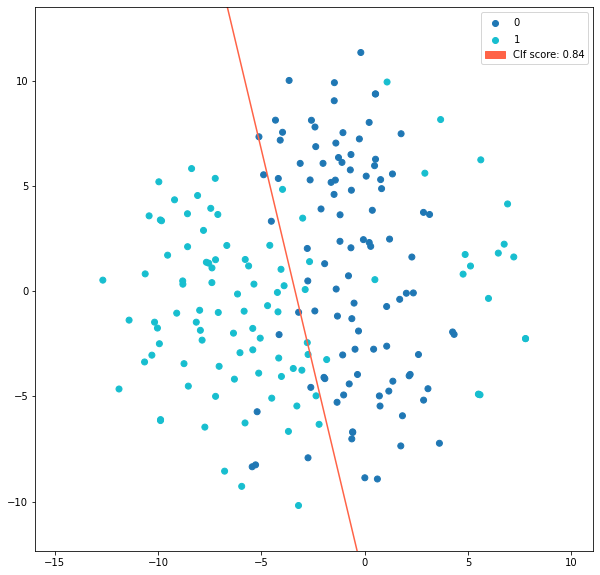
\includegraphics[width=\textwidth]{Figures/transfer-finetuned.png}
            \caption{Finetune}
            \label{fig:finetune}
          \end{subfigure}
          \hfill
          \begin{subfigure}[b]{0.49\columnwidth}
            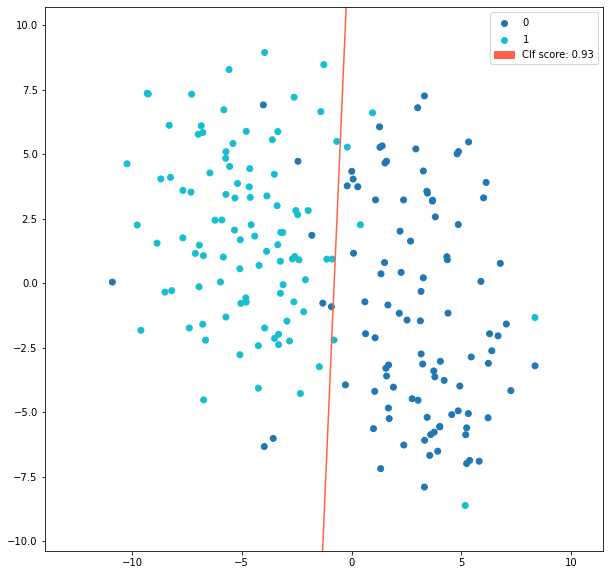
\includegraphics[width=\textwidth]{Figures/transfer-augmented.png}
            \caption{Finetune + Data Augmentation}
            \label{fig:augmentation}
          \end{subfigure}
          \caption{\emph{t-SNE} representation of the Alien vs Predator dataset. Linear classifier in each of them.}
          \label{fig:four figures}
        \end{figure}
        The accuracy scores obtained by each of the linear models are presented in Table \ref{table:tsne:transfer}.
        \begin{table}[H]
          \begin{tabular}{l|llll}
                     & Trained from zero       & Pretrained + SVM         & \begin{tabular}[c]{@{}l@{}}Finetuning (no data\\ augmentation)\end{tabular} & Finetuning (data augmentation) \\ \hline
            Accuracy & \multicolumn{1}{r}{0.7} & \multicolumn{1}{r}{0.79} & \multicolumn{1}{r}{0.84}                                                    & \multicolumn{1}{r}{0.93}
          \end{tabular}
          \caption{Obtained results linear classification of \emph{t-SNE} representation in Alien vs Predator dataset.}
          \label{table:tsne:transfer}
        \end{table}
        The analysis using the images or the tables is quite similar. As we can observe, the representations obtained using the trained from scratch model are quite bad (Figure \ref{fig:scratch}). It is linearly separated in the bottom part of the image, but in general the points of the different classes are mixed. When we use a pretrained model with a SVM on top (Figure \ref{fig:svm}) the linear separability improves a little bit, we can see how the majority of the class \(1\) points are below the separating hyperplane and the opposite happens with the points of class \(0\). Still, there is margin for improvement. Finetuning the model (Figure \ref{fig:finetune}) leads to a quite accurate separation,but we still have some noise on the separating hyperplane. In the last iteration, using data augmentation (Figure \ref{fig:augmentation}), we obtain the most linearly separable case obtaining a \(0.93\) accuracy score using a linear classifier, which is a reasonable result.

        In general, we can state that \textbf{training from zero} is not a good idea since we need much more epochs to converge to a solution and, if the network has a great number of parameters, it could lead to overfitting. The representations obtained by \emph{t-SNE} get more linearly separable when we use \textbf{transfer learning with finetuning}, getting to its highest accuracy when data augmentation is added.
\end{itemize}
\end{document}